
%(BEGIN_QUESTION)
% Copyright 2012, Tony R. Kuphaldt, released under the Creative Commons Attribution License (v 1.0)
% This means you may do almost anything with this work of mine, so long as you give me proper credit

A technician performs a valve ``scan'' using the diagnostic capabilities of a smart valve positioner, obtaining this ``signature'' plot as a result:

$$\includegraphics[width=15.5cm]{i01917x01.eps}$$

Approximate the amount of work done by the pneumatic actuator in lifting the valve stem from its fully-closed to its fully-open position.  The valve is a Fisher E-body with cage-guided trim (equal-percentage characteristic), a full-open $C_v$ of 35.7, and a type 667 actuator with a diaphragm diameter of 14 inches.  The positioner's air supply pressure is 45 PSI.

\vskip 10pt

Work $\approx$ \underbar{\hskip 50pt} ft-lbs

\vskip 10pt

If we had some way to eliminate any and all friction from this control valve's mechanism, what effect would this elimination have on the amount of work necessary to fully open the valve?  Would the amount of required work {\it increase}, {\it decrease}, or {\it remain the same} as it is now?

\vskip 10pt

Is this control valve assembly {\it fail-open} or is it {\it fail-closed} (assuming a lift-to-open valve body)?

\underbar{file i01917}
%(END_QUESTION)





%(BEGIN_ANSWER)

Award 5 points for a correct work approximation ($\pm$ 2\%), 3 points for friction effect, and 2 points for fail mode.

\vskip 10pt

Work $\approx$ {\bf 205} ft-lb ($\pm$ 5 ft-lb) -- {\it Converting the vertical scale into pounds of force using $F = PA$, the area underneath the function is equivalent to work in units of inch-pounds.  The rectangular section (6 PSI high by 1 inch wide) is equivalent to 923.6 inch-pounds of work, while the triangular section (20 PSI high by 1 inch wide) is equivalent to 1539.4 inch-pounds of work.  Together their combined area is 2463.0 inch-pounds of work, or 205.25 foot-pounds of work.}

\vskip 10pt

Without friction, the amount of work necessary will {\bf decrease}.

\vskip 10pt

This is a {\bf fail-closed} control valve.

%(END_ANSWER)





%(BEGIN_NOTES)

{\bf This question is intended for exams only and not worksheets!}.

%(END_NOTES)


